\subsubsection{Rotação de Pontos no Plano Cartesiano}

\begin{definition}
Considere o ponto $A = (x, y) \in \R^2$ e chame de $\alpha$ o ângulo
formado pelo segmento $OA$ com o eixo positivo de $x$. A função
$T_{\theta} : \R^2 \to \R^2$  tal que
$$T_{\theta}\paren{x, y} = \paren{x\cdot \cos \theta - y\cdot \sen \theta, x\cdot \sen \theta + y\cdot \cos
\theta}$$ é a rotação de ângulo $\theta$ do ponto $A = (x,y)$ em
torno da origem.
%
\begin{figure}
\centering
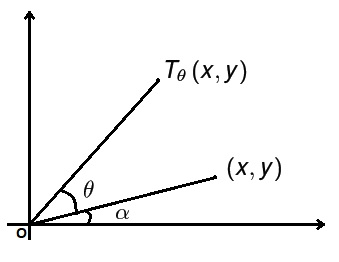
\includegraphics[width=5.5cm]{\imgdirfromsection/rotacao.jpg}
\end{figure}
    
\end{definition}

\begin{onlineact}
    \khan{https://pt.khanacademy.org/math/trigonometry/trig-equations-and-identities/intro-to-trig-angle-addition-identities/e/trig_addition_identities}
    {Uso das Identidades Trigonométricas de Soma de Ângulos}.
\end{onlineact}

\begin{onlineact}
    \khan{https://pt.khanacademy.org/math/trigonometry/trig-equations-and-identities/using-trig-identities/e/applying-angle-addition-formulas}
    {Calcule Valores Trigonométricos a Partir de Identidades de Soma de Ângulos}.
\end{onlineact}